\chapter{数据库设计}
\section{数据库环境说明}
本系统的数据系统采用Oracle数据库系统,并基于关系数据库进行扩展\\
扩展部分结合非关系型数据库NoSQL实现\\
扩展原因为:\\
由于即时通讯中需要存储音频与视频,需要存储多媒体数据\\
多媒体数据与传统数据库数据有显著的不同,多媒体数据库有以下特点。\\
1)数据量巨大且媒体之间量的差异十分明显,而使得数据在库中的组织方法和存储方法复杂。\\
2)媒体种类的繁多使得数据处理变得非常复杂。\\
3)多媒体不仅改变了数据库的接口,使其声、图、文并茂,而且也改变了数据库的操纵形式,其中最重要的是查询机制和查询方法。媒体的复合、分散、时序性质及其形象化的特点,使得查询不再只是通过字符查询,查询的结果也不仅是一张表,而是多媒体的一组“表现”。接口的多媒体化将对查询提出更复杂、更友好的设计要求



\section{数据库的命名规则}
\begin{itemize}
    \item 1. 实体的命名方式为驼峰命名
    \item 2. 允许单词缩写,很长的单词可以采取前几个字母作为代表
    \item 3. 属性名采用小写命名的方式,可以通过下划线添加备注前缀
    \item 4. 字段不带类型前缀
    \item 5. 实体表名为单数
    \item 6. 关联表表名命名方法:将两个表名字的全称或缩写用下划线连接起来,对于两个实体间的多种关系,加入表示该关系的后缀
    \item 7. 字符数限制:20
\end{itemize}

\section{逻辑设计}
是否需要满足某一种范式。
        \begin{figure}[ht]
            \centering
            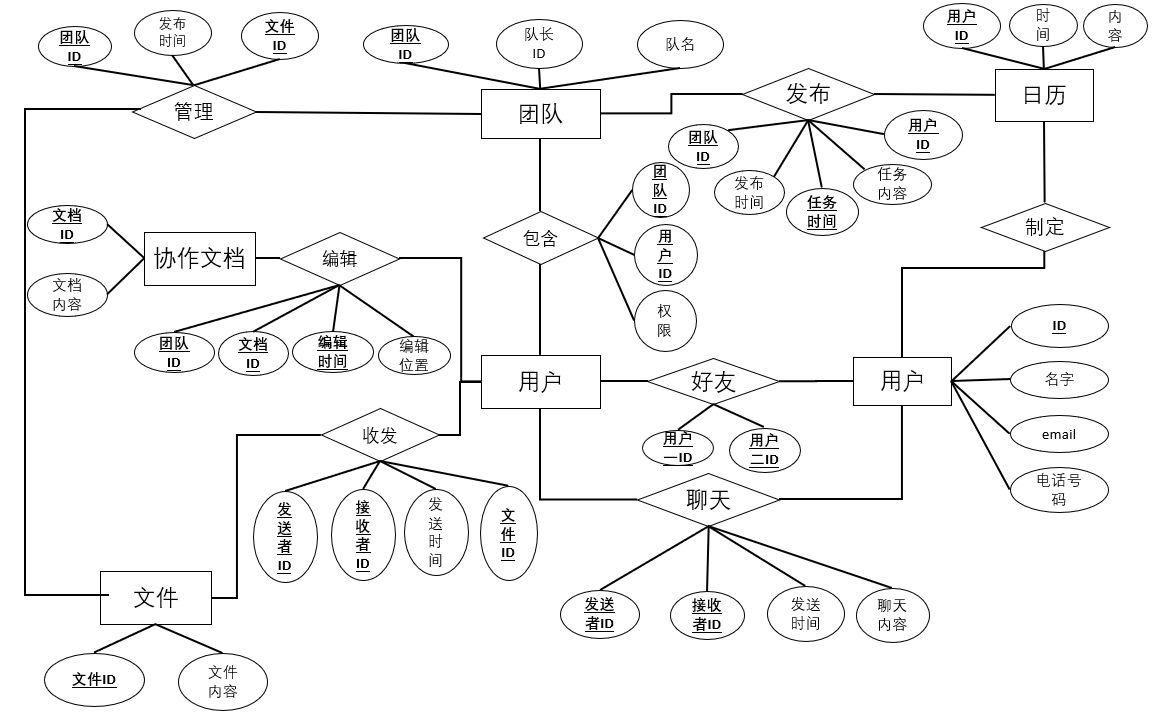
\includegraphics[scale =0.6]{数据库.png}\label{tab:classification}
            \caption{数据库逻辑图}\label{fig:noted-figure}
        \end{figure}
        \newpage
画个实体的逻辑关系表/图在此处。

\section{物理设计}
\subsection{数据库产品}
采用Oracle数据库和Hbase分布式数据库结合。\\
采用Oracle集中数据库存储文件,用户信息。\\
采用分布式数据库Hbase(NoSQL)存储聊天信息,多媒体信息。\\

集中存储用户信息,文件有利于数据管理,分析,隐私保护\\
分布存储有利于系统性能提升,且可避免单点失效导致服务丢失。\\

\subsection{实体属性、类型、精度}
\subsubsection{用户数据表设计}
\begin{table}[htbp]
\centering
\caption{用户数据表User设计} \label{tab:client-database}
\begin{tabular}{|c|c|c|c|c|}
    \hline
    字段名 & 类型 & 大小 & 说明 & 备注 \\
    \hline
    id & char & 64 & 用户的唯一标识符 & 主键\\
    \hline
    name & char & 64 & 用户的名字 & · \\
    \hline
    email & char  & 64 & 用户的电子邮箱 & · \\
    \hline
    phone & char & 11 & 用户的联系电话 & · \\
    \hline
\end{tabular}
\note{用户数据表User设计}
\end{table}
%========================================
\subsubsection{团队数据表设计}
\begin{table}[htbp]
\centering
\caption{团队数据表Group设计} \label{tab:order-database}
\begin{tabular}{|c|c|c|c|c|}
    \hline
    字段名 & 类型 & 大小 & 说明 & 备注 \\
    \hline
    group\_id & char & 64 & 团队的唯一标识符 & 主键\\
    \hline
    leader\_id & char & 64 & 队长的ID & 外键,来自用户表 \\
    \hline
    name & char & 64 & 团队的名字 & · \\
    \hline
\end{tabular}
\note{团队数据表Group设计}
\end{table}
%========================================
\subsubsection{日历数据表设计}
\begin{table}[htbp]
\centering
\caption{日历数据表Calendar设计} \label{tab:order-database}
\begin{tabular}{|c|c|c|c|c|}
    \hline
    字段名 & 类型 & 大小 & 说明 & 备注 \\
    \hline
    id & char & 64 & 日历的唯一标识符 & 主键\\
    \hline
    time & time & 4 & 日历中任务的时间 & · \\
    \hline
    task & char & 512 & 日历中任务的内容 & · \\
    \hline
\end{tabular}
\note{日历数据表Calendar设计}
\end{table}
%========================================
\subsubsection{文件数据表设计}
\begin{table}[htbp]
\centering
\caption{文件数据表File设计} \label{tab:order-database}
\begin{tabular}{|c|c|c|c|c|}
    \hline
    字段名 & 类型 & 大小 & 说明 & 备注 \\
    \hline
    id & char & 64 & 文件的唯一标识符 & 主键\\
    \hline
    file & char & 10G & 文件的内容 & · \\
    \hline
\end{tabular}
\note{文件数据表File设计}
\end{table}
%========================================
\subsubsection{协作文档数据表设计}
\begin{table}[htbp]
\centering
\caption{协作文档数据表Coop设计} \label{tab:order-database}
\begin{tabular}{|c|c|c|c|c|}
    \hline
    字段名 & 类型 & 大小 & 说明 & 备注 \\
    \hline
    id & char & 64 & 文档的唯一标识符 & 主键\\
    \hline
    doc & char & 10G & 在线协作文档的内容 & · \\
    \hline
\end{tabular}
\note{协作文档数据表Coop设计}
\end{table}
%========================================
\subsubsection{团队-用户关系数据表设计}
\begin{table}[htbp]
\centering
\caption{包含关系数据表Group\_User} \label{tab:order-database}
\begin{tabular}{|c|c|c|c|c|}
    \hline
    字段名 & 类型 & 大小 & 说明 & 备注 \\
    \hline
    group\_id & char & 64 & 包含关系的标识符之一 & 主键|外键,来自团队表
    \\
    \hline
    user\_id & char & 64 & 包含关系的标识符之一 & 主键|外键,来自用户表 \\
    \hline
    name & char & 64 & 团队的名字 & · \\
    \hline
\end{tabular}
\note{团队-用户包含关系数据表Group\_User设计}
\end{table}
%========================================
\subsubsection{团队-日历关系数据表设计}
\begin{table}[htbp]
\centering
\caption{发布关系数据表Group\_Calendar} \label{tab:order-database}
\begin{tabular}{|c|c|c|c|c|}
    \hline
    字段名 & 类型 & 大小 & 说明 & 备注 \\
    \hline
    group\_id & char & 64 & 发布关系的标识符之一 & 主键|外键,来自团队表
    \\
    \hline
    user\_id & char & 64 & 发布关系的标识符之一 & 主键|外键,来自用户表
    \\
    \hline
    task\_time & time & 4 & 发布关系的标识符之一 & 主键\\
    \hline
    issue\_time & time & 4 & 发布任务的时间 & · \\
    \hline
    task & char & 512 & 发布任务的内容 & · \\  
    \hline
\end{tabular}
\note{团队-日历发布关系数据表Group\_Calendar设计}
\end{table}
%========================================
\subsubsection{团队-文件关系数据表设计}
\begin{table}[htbp]
\centering
\caption{管理关系数据表Group\_File} \label{tab:order-database}
\begin{tabular}{|c|c|c|c|c|}
    \hline
    字段名 & 类型 & 大小 & 说明 & 备注 \\
    \hline
    group\_id & char & 64 & 管理关系的标识符之一 & 主键|外键,来自团队表
    \\
    \hline
    file\_id & char & 64 & 管理关系的标识符之一 & 主键|外键,来自文件表
    \\
    \hline
    time & time & 4 & 发布文件的时间 & · \\ 
    \hline
\end{tabular}
\note{团队-文件管理关系数据表Group\_File设计}
\end{table}
%========================================
\subsubsection{用户-协作文档关系数据表设计}
\begin{table}[htbp]
\centering
\caption{编辑关系数据表User\_Coop} \label{tab:order-database}
\begin{tabular}{|c|c|c|c|c|}
    \hline
    字段名 & 类型 & 大小 & 说明 & 备注 \\
    \hline
    user\_id & char & 64 & 编辑关系的标识符之一 & 主键|外键,来自用户表
    \\
    \hline
    file\_id & char & 64 & 编辑关系的标识符之一 & 主键|外键,来自协作文档表 \\
    \hline
    edit\_time & time & 4 & 编辑关系的标识符之一 & 主键 \\ 
    \hline
    edit\_pos & int & 4 & 编辑的位置 & · \\ 
    \hline
\end{tabular}
\note{用户-协作文档编辑关系数据表User\_Coop设计}
\end{table}
%========================================
\subsubsection{用户-用户关系数据表设计}
\begin{table}[htbp]
\centering
\caption{好友关系数据表User\_User\_Friend} \label{tab:order-database}
\begin{tabular}{|c|c|c|c|c|}
    \hline
    字段名 & 类型 & 大小 & 说明 & 备注 \\
    \hline
    id1 & char & 64 & 好友关系的标识符之一 & 主键|外键,来自用户表 \\
    \hline
    id2 & char & 64 & 好友关系的标识符之一 & 主键|外键,来自用户表 \\
    \hline
\end{tabular}
\note{好友关系数据表User\_User\_Friend设计}
\end{table}

\begin{table}[htbp]
\centering
\caption{聊天关系数据表User\_User\_Chat} \label{tab:order-database}
\begin{tabular}{|c|c|c|c|c|}
    \hline
    字段名 & 类型 & 大小 & 说明 & 备注 \\
    \hline
    send\_id & char & 64 & 聊天关系的标识符之一 & 主键|外键,来自用户表 \\
    \hline
    recv\_id & char & 64 & 聊天关系的标识符之一 & 主键|外键,来自用户表 \\
    \hline
    time & time & 4 & 聊天信息的发送时间 & · \\ 
    \hline
    message & char & 512 & 聊天内容 & · \\ 
    \hline
\end{tabular}
\note{聊天关系数据表User\_User\_Chat设计}
\end{table}
%========================================
\subsubsection{用户-文件关系数据表设计}
\begin{table}[htbp]
\centering
\caption{收发关系数据表User\_File} \label{tab:order-database}
\begin{tabular}{|c|c|c|c|c|}
    \hline
    字段名 & 类型 & 大小 & 说明 & 备注 \\
    \hline
    send\_id & char & 64 & 收发关系的标识符之一 & 主键|外键,来自用户表 \\
    \hline
    recv\_id & char & 64 & 收发关系的标识符之一 & 主键|外键,来自用户表 \\
    \hline
    file\_id & char & 64 & 收发关系的标识符之一 & 主键|外键,来自文件表 \\
    \hline
    time & time & 4 & 文件的发送时间 & · \\ 
    \hline
\end{tabular}
\note{用户-文件收发关系数据表User\_File设计}
\end{table}



\newpage

\section{安全性设计}
安全性设计主要包括容灾和备份设计。容灾是为了在遭遇灾害时能保证信息系统能正常运行,从而实现业务连续性;备份是为了应对灾难来临时造成的数据丢失问题。

对于即时通讯系统,由于其用户群体巨大且即时通讯需求强,因此遭遇灾害时迅速恢复是至关重要的设计;此外对于用户尤其是企业级用户,文件及数据的机密性,可靠性,可用性等必须通过备份保证。

\subsection{备份设计}
\begin{itemize}
\item 按空间分类,分别进行同城和异地备份。\\
同城备份将数据备份在本地,其特点是速度相对较快。缺点是一旦发生大灾大难,将无法保证本地容灾备份机房中的数据和系统仍可用。
异地备份,通过互联网TCP/IP协议,将生产中心的数据备份到异地。具体而言,备份到300公里以外,并且不能在同一地震带,不能在同地电网,不能在同一江河流域。这样即使发生大灾大难,也可以在异地进行数据回退。采用远程备份技术和快照技术。

\item 按时间分类,每天,每周进行不同级别的备份。\\
1. 每周对数据库进行一次完全备份。\\
2. 每天夜里2:00 am -3:00 am 对数据库的事务日志进行差异备份。\\
3. 在异地建立一个热备份点,通过网络进行同步数据备份。也就是通过网络以同步方式,把主站点的数据备份到备份站点,备份站点一般只备份数据,不承担业务。当出现灾难时,备份站点接替主站点的业务,从而维护业务运行的连续性。\\
\end{itemize}

\subsection{容灾设计}
容灾系统可以分为数据容灾和应用容灾,其实现如下:
\begin{itemize}
     
\item 数据容灾要求建立一个异地的数据系统,该系统是本地关键应用数据的一个实时复制。在本地数据及整个应用系统出现灾难时,系统至少在异地保存有一份可用的关键业务的数据。采用同步传输方式。

\item 应用容灾要求在异地建立一套完整的与本地生产系统相当的备份应用系统(可以是互为备份),在灾难情况下,远程系统迅速接管业务运行。其不仅需要一份可用的数据复制,还要有包括网络、主机、应用、甚至IP等资源,以及各资源之间的良好协调。主要的技术包括负载均衡、集群技术。

\item 需要高可靠性软件协调应用的切换 \\
高可靠性软件用于自动检测系统的运行状态,在一台服务器出现故障的情况下,自动地把设定的服务转到另一台服务器上。当运行服务器提供的服务不可用时,备份服务器自动接替运行服务器的工作而不用重新启动系统,而当运行服务器恢复正常后,按照使用者的设定以自动或手动方式将服务切换到运行服务上运行。
\end{itemize}
\section{数据库管理与维护说明}
对于数据库的维护,随时对数据库中的信息加以调试和保存备份。同样需要个工作人员进行系统的分析和用户的反馈,对系统进行升级以及功能的完善。同时保证系统安全有序的运行。